\documentclass[twocolumn]{article}

\usepackage{listings}										
\usepackage{graphicx}									

\title{Lab#2\\Computational Physics I - Phys381}		
\author{Guilherme Contesini , 10140201 \\ Gerswin Magat , 00325287}		

\begin{document}
\maketitle																
\onecolumn
{
\begin{abstract} \textbf{A Case Study: Patriot Missile System} \newline
On February 25, 1991, a Patriot missile defence system operating at Dhahran, Saudi Arabia, during Operation Desert Storm failed to track and intercept an incoming Scud. This Scud subsequently hit an Army barracks, killing 28 Americans. This report responds to your request that we review the facts associated with this incident and determine if a computer software problem was involved. \newline

...The Patriot battery at Dhahran failed to track and intercept the Scud missile because of a software problem in the system's weapons control computer. This problem led to an inaccurate tracking calculation that became worse the longer the system operated. At the time of the incident, the battery had been operating continuously for over 100 hours. By then, the inaccuracy was serious enough to cause the system to look in the wrong place for the incoming Scud. Two weeks before the incident, Army officials received Israeli data indicating some loss in accuracy after the system had been running for 8 consecutive hours. Consequently, Army officials modified the software to improve the system's accuracy. However, the modified software did not reach Dhahran until February 26, 1991--the day after the Scud incident. \newline

\footnotesize{- An excerpt from a report by the United States General Accounting Office, Information Management and Technology Division, in Washington, D.C., February 4, 1992}

\end{abstract} 
}
\twocolumn
\newpage														

%%%%%%%%%%%%%%%%%%%%%%%%%%%%%%%%%%%%%%%%%%%%%%%%%%%%%%%%%%%%%%%%%%%%%%%%%%%%%%%%%%%%%%%%%%%%%%%%%%%%%%%%%%%%%%%%%%%%%%%%

\section{Truncated Error Function}													

%%%%%%%%%%%%%%%%%%%%%%%%%%%%%%%%%%%%%%%%%%%%%%%%%%%%%%%%%%%%%%%%%%%%%%%%%%%%%%%%%%%%%%%%%%%%%%%%%%%%%%%%%%%%%%%%%%%%%%%%

\subsection{i:}														
%%%%%%%%%%%%%%%%%%%%%%%%%%%%%%%%%%%%%%%%%%%%%%%%%%%%%%%%%%%%%%%%%%%%%%%%%%%%%%%%%%%%%%%%%%%%%%%%%%%%%%%%%%%%%%%%%%%%%%%%
\subsubsection{a:}		
\begin{verbatim}
  function horner(coef_aux_vector, 
x_dp) result (result_dp)
    implicit none
    double precision , dimension (:) ,
 intent (in) :: coef_aux_vector
    double precision , intent (in) ::
 x_dp
    real :: result_dp
    integer :: i_int , k_int
    result_dp = 0.0
    i_int = 0
    do k_int = 1 , size(coef_aux_vector)
 , 1
      result_dp = result_dp + 
coef_aux_vector(k_int) * x_dp**(2*i_int)
      i_int = i_int + 1
    end do
  end function
\end{verbatim}
%%%%%%%%%%%%%%%%%%%%%%%%%%%%%%%%%%%%%%%%%%%%%%%%%%%%%%%%%%%%%%%%%%%%%%%%%%%%%%%%%%%%%%%%%%%%%%%%%%%%%%%%%%%%%%%%%%%%%%%%
\subsubsection{b:}
\begin{verbatim}
  recursive function fact( k ) 
result ( factor )
    implicit none
    integer, intent(in):: k
    double precision :: factor
    if(k == 0) then
      factor = 1
    else
      factor = k * fact( k-1 )
    endif
  end function
\end{verbatim}
%%%%%%%%%%%%%%%%%%%%%%%%%%%%%%%%%%%%%%%%%%%%%%%%%%%%%%%%%%%%%%%%%%%%%%%%%%%%%%%%%%%%%%%%%%%%%%%%%%%%%%%%%%%%%%%%%%%%%%%%
\subsubsection{c:}	
\begin{verbatim}
erf(x)
\end{verbatim}									%%%%%%%%%%%%%%%%%%%%%%%%%%%%%%%%%%%%%%%%%%%%%%%%%%%%%%%%%%%%%%%%%%%%%%%%%%%%%%%%%%%%%%%%%%%%%%%%%%%%%%%%%%%%%%%%%%%%%%%%
\subsection{ii:}		
\onecolumn
{
Figure obtained through the [{~\ref{[phys381erf.f90]}}] and plotted using [~\ref{[phys381erf.gp]}]:\\
\begin{figure}[!h]
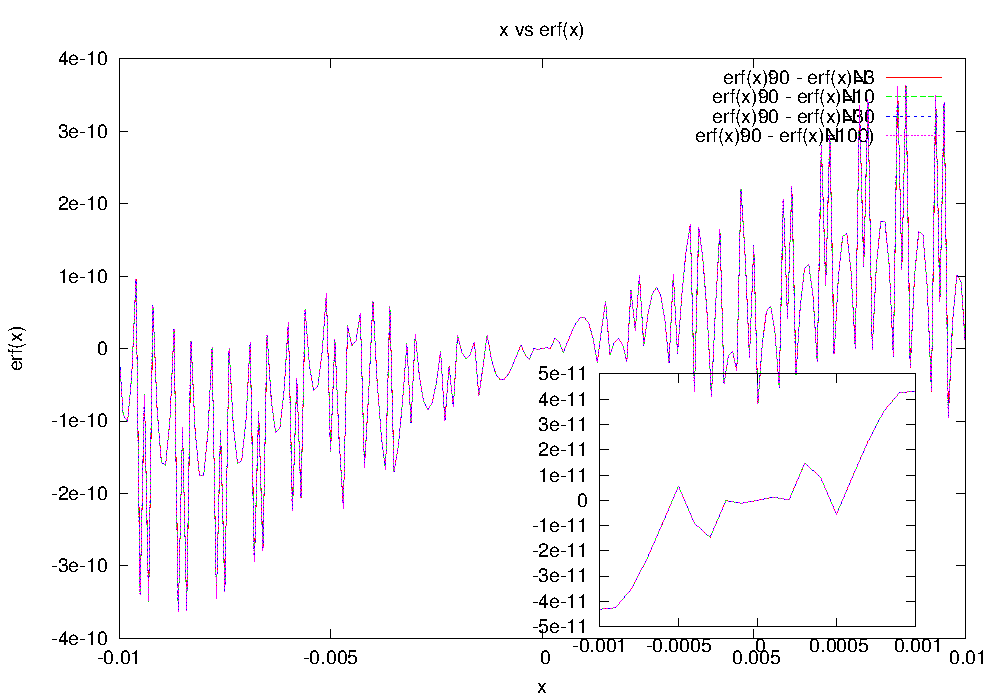
\includegraphics[width=1.1\textwidth]{Plot1.png}
\end{figure}
}
\twocolumn
%%%%%%%%%%%%%%%%%%%%%%%%%%%%%%%%%%%%%%%%%%%%%%%%%%%%%%%%%%%%%%%%%%%%%%%%%%%%%%%%%%%%%%%%%%%%%%%%%%%%%%%%%%%%%%%%%%%%%%%%
\subsection{iii:}
I don't see any difference but I believe that with a between 30 and 100 would be a perfect choice.
%%%%%%%%%%%%%%%%%%%%%%%%%%%%%%%%%%%%%%%%%%%%%%%%%%%%%%%%%%%%%%%%%%%%%%%%%%%%%%%%%%%%%%%%%%%%%%%%%%%%%%%%%%%%%%%%%%%%%%%%
\subsection{iv:}	
\onecolumn
{
Figure obtained through the [{~\ref{[phys381erf.f90]}}] and plotted using [~\ref{[phys381erf.gp]}]:\\
\begin{figure}[!h]
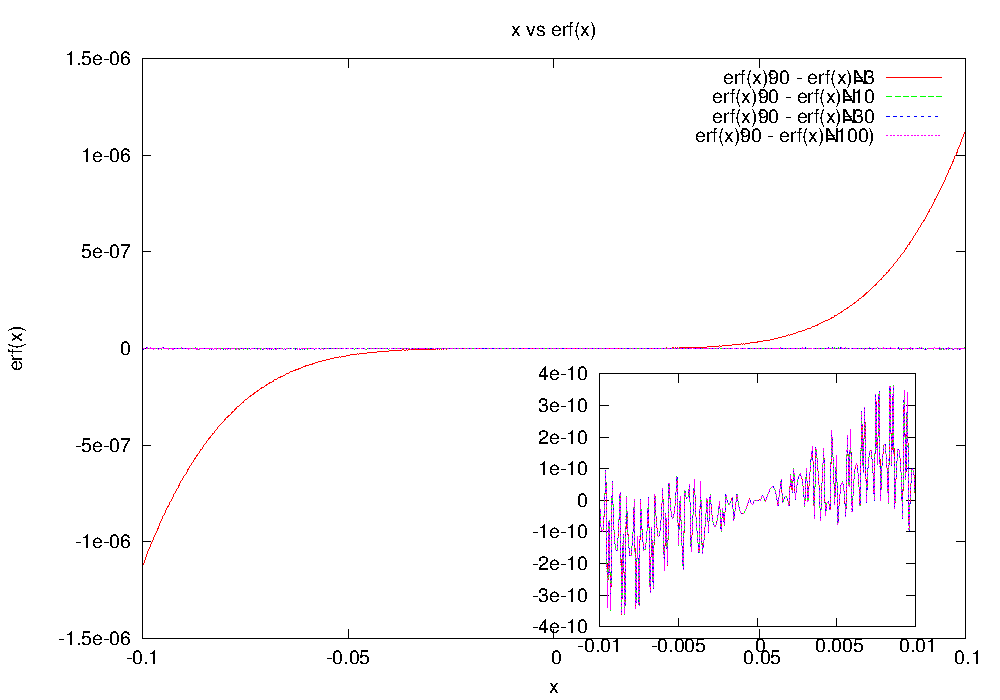
\includegraphics[width=1.1\textwidth]{Plot2.png}
\end{figure}
}
\onecolumn
{
\begin{figure}[!h]
\includegraphics[width=1.1\textwidth]{Plot3.png}
\end{figure}
}

note : you will only see changes when $ |x| > 2 $ as showed in figure 3
%%%%%%%%%%%%%%%%%%%%%%%%%%%%%%%%%%%%%%%%%%%%%%%%%%%%%%%%%%%%%%%%%%%%%%%%%%%%%%%%%%%%%%%%%%%%%%%%%%%%%%%%%%%%%%%%%%%%%%%%
\subsection{The complementary error function:}
%%%%%%%%%%%%%%%%%%%%%%%%%%%%%%%%%%%%%%%%%%%%%%%%%%%%%%%%%%%%%%%%%%%%%%%%%%%%%%%%%%%%%%%%%%%%%%%%%%%%%%%%%%%%%%%%%%%%%%%%
\subsubsection{i:}			
\begin{verbatim}
  function new_erfc( x_dp ) result ( erf_dp )
    implicit none
    	integer , intent(in) :: n_int
    double precision , intent(in) :: x_dp
    integer :: k_int   
    double precision :: erf_dp , pi , i_int
    double precision , allocatable , dimension(:) :: coef_vector 
    i_int = 0
    erf_dp = 0.
    pi= 4*atan(1.)
    allocate(coef_vector(n_int))
    do k_int = 1 , size(coef_vector) , 1
      coef_vector(k_int) = ((-1**i_int)*fact(fact(2*i_int-1)))
      i_int = i_int + 1
    end do
    erf_dp = ( exp(((-1*x_dp)**2 )) / ((x_dp)*(sqrt(pi) ))) * horner( coef_vector , (2*x_dp)**(-1) )
    deallocate(coef_vector)
  end function
\end{verbatim}											
%%%%%%%%%%%%%%%%%%%%%%%%%%%%%%%%%%%%%%%%%%%%%%%%%%%%%%%%%%%%%%%%%%%%%%%%%%%%%%%%%%%%%%%%%%%%%%%%%%%%%%%%%%%%%%%%%%%%%%%%
\subsubsection{ii:}														
%%%%%%%%%%%%%%%%%%%%%%%%%%%%%%%%%%%%%%%%%%%%%%%%%%%%%%%%%%%%%%%%%%%%%%%%%%%%%%%%%%%%%%%%%%%%%%%%%%%%%%%%%%%%%%%%%%%%%%%%
\subsubsection{iii:}														
%%%%%%%%%%%%%%%%%%%%%%%%%%%%%%%%%%%%%%%%%%%%%%%%%%%%%%%%%%%%%%%%%%%%%%%%%%%%%%%%%%%%%%%%%%%%%%%%%%%%%%%%%%%%%%%%%%%%%%%%
%%%%%%%%%%%%%%%%%%%%%%%%%%%%%%%%%%%%%%%%%%%%%%%%%%%%%%%%%%%%%%%%%%%%%%%%%%%%%%%%%%%%%%%%%%%%%%%%%%%%%%%%%%%%%%%%%%%%%%%%
\section{Conclusion:}
%%%%%%%%%%%%%%%%%%%%%%%%%%%%%%%%%%%%%%%%%%%%%%%%%%%%%%%%%%%%%%%%%%%%%%%%%%%%%%%%%%%%%%%%%%%%%%%%%%%%%%%%%%%%%%%%%%%%%%%%
\section{Codes:}
\subsection{phys381erf.f90}\label{[phys381erf.f90]}

note : the algorithm for step iv  is the same with a small difference in the main loop, starting this time on num_dp= -0.1 and ending in num_dp = 0.1 .
\begin{verbatim}
program phys381erf

  implicit none
  integer :: j_int 
  double precision :: num_dp , 
value_float
  open( 12 , file = "erfout.data")

  num_dp = -0.01
  do j_int = -100 , 100 , 1
    write(12,*) num_dp , erf(num_dp) 
,new1_erf(num_dp) , new2_erf(num_dp) 
, new3_erf(num_dp) , new4_erf(num_dp)
    write(*,*) num_dp , j_int
    num_dp = num_dp + 0.0001
  end do

contains

  function new1_erf( x_dp ) 
result ( erf_dp )

    implicit none
    double precision , intent(in) ::
 x_dp
    integer :: k_int , n_int , i_int
    double precision :: erf_dp , pi 
    double precision , allocatable ,
 dimension(:) :: coef_vector 

    n_int = 2
    i_int = 0
    erf_dp = 0.
    pi= 4*atan(1.)
    allocate(coef_vector(n_int))
    do k_int = 1 , size(coef_vector) , 1
      coef_vector(k_int) = (((-1)**
(i_int))/(fact(i_int)*(2*i_int+1)))
      i_int = i_int + 1
    end do

    erf_dp = ((2*x_dp)/sqrt(pi)) 
* horner( coef_vector , x_dp )

    deallocate(coef_vector)
  end function

  function new2_erf( x_dp ) 
result ( erf_dp )

    implicit none
    double precision , intent(in) ::
 x_dp
    integer :: k_int , n_int , i_int
    double precision :: erf_dp , pi 
    double precision , allocatable ,
 dimension(:) :: coef_vector 

    n_int = 9
    i_int = 0
    erf_dp = 0.
    pi= 4*atan(1.)
    allocate(coef_vector(n_int))
    do k_int = 1 , size(coef_vector) , 1
      coef_vector(k_int) = (((-1)**
(i_int))/(fact(i_int)*(2*i_int+1)))
      i_int = i_int + 1
    end do

    erf_dp = ((2*x_dp)/sqrt(pi)) * 
horner( coef_vector , x_dp )

    deallocate(coef_vector)
  end function

  function new3_erf( x_dp ) 
result ( erf_dp )

    implicit none
    double precision , intent(in) ::
 x_dp
    integer :: k_int , n_int , i_int
    double precision :: erf_dp , pi 
    double precision , allocatable ,
 dimension(:) :: coef_vector 

    n_int = 29
    i_int = 0
    erf_dp = 0.
    pi= 4*atan(1.)
    allocate(coef_vector(n_int))
    do k_int = 1 , size(coef_vector) , 1
      coef_vector(k_int) = (((-1)**
(i_int))/(fact(i_int)*(2*i_int+1)))
      i_int = i_int + 1
    end do

    erf_dp = ((2*x_dp)/sqrt(pi)) * 
horner( coef_vector , x_dp )

    deallocate(coef_vector)
  end function

  function new4_erf( x_dp ) 
result ( erf_dp )

    implicit none
    double precision , intent(in) :: x_dp
    integer :: k_int , n_int , i_int
    double precision :: erf_dp , pi 
    double precision , allocatable ,
 dimension(:) :: coef_vector 

    n_int = 99
    i_int = 0
    erf_dp = 0.
    pi= 4*atan(1.)
    allocate(coef_vector(n_int))
    do k_int = 1 , size(coef_vector) , 1
      coef_vector(k_int) = (((-1)**
(i_int))/(fact(i_int)*(2*i_int+1)))
      i_int = i_int + 1
    end do

    erf_dp = ((2*x_dp)/sqrt(pi)) *
 horner( coef_vector , x_dp )

    deallocate(coef_vector)
  end function

  recursive function fact( k ) 
result ( factor )

    implicit none
    integer, intent(in):: k
    double precision :: factor

    if(k == 0) then
      factor = 1
    else
      factor = k * fact( k-1 )
    endif

  end function

  function horner(coef_aux_vector, 
x_dp) result (result_dp)

    implicit none
    double precision , dimension (:) ,
 intent (in) :: coef_aux_vector
    double precision , intent (in) ::
 x_dp
    real :: result_dp
    integer :: i_int , k_int

    result_dp = 0.0
    i_int = 0
    do k_int = 1 , size(coef_aux_vector)
 , 1
      result_dp = result_dp + 
coef_aux_vector(k_int) * x_dp**(2*i_int)
      i_int = i_int + 1
    end do

  end function
end program 
\end{verbatim}
\subsection{phys381erf.gp}\label{[phys381erf.gp]}
\begin{verbatim}
reset
set terminal png size 1700,1500
set output "Plot1.png"
set multiplot 
set autoscale
set size 0.5,0.3333

set origin 0.25, 0.6666
set title 'erf(x)@f90 vs X'
set xlabel 'x'
set ylabel 'erf(x)'
plot 'erfout.data' u 1:2 with l
 notitle

set origin 0.5 , 0.0
set title 'erf(x)@f90 - erf(x)@N=3'
set xlabel 'x'
set ylabel 'erf(x)@f90 - erf(x)@N=3'
plot 'erfout.data' u 1:($3-$2) with l
 notitle

set origin 0.0, 0.0
set title 'erf(x)@f90 - erf(x)@N=10'
set xlabel 'x'
set ylabel 'erf(x)@f90 - erf(x)@N=10'
plot 'erfout.data' u ($1):($4-$2) 
with l notitle

set origin 0.0, 0.3333
set title 'erf(x)@f90 - erf(x)@N=30'
set xlabel 'x'
set ylabel 'erf(x)@f90 - erf(x)@N=30'
plot 'erfout.data' u ($1):($5-$2) 
with l notitle

set origin 0.5 , 0.3333
set title 'erf(x)@f90 - erf(x)@N=100'
set xlabel 'x'
set ylabel 'erf(x)@f90 - erf(x)@N=100)'
plot 'erfout.data' u ($1):($6-$2) 
with l notitle

reset
\end{verbatim}

\begin{verbatim}
program phys381erfpart2

  implicit none
  integer :: j_int 
  double precision :: num_dp , value_float
  open( 12 , file = "erfout2.data")

!-------------------------------------------------------------------------------
  num_dp = 2.5

  do j_int = 2 , 20 , 1
    write(12,*) j_int , erfc(num_dp) ,new_erf(num_dp , j_int )
  end do

!!!!!!!!!!!!!!!!!!!!!!!!!!!!!!!!!!!!!!!!!!!!!!!!!!!!!!!!!!!!!!!!!!!!!!!!!!!!!!!!

contains

  function new_erfc( x_dp ) result 
  ( erf_dp )
  
    implicit none
    double precision , intent(in) ::
     x_dp
    integer :: k_int , n_int 
    double precision :: erf_dp , pi ,
     i_int
    double precision , allocatable , 
    dimension(:) :: coef_vector 

    n_int = 19
    i_int = 0
    erf_dp = 0.
    pi= 4*atan(1.)
    allocate(coef_vector(n_int))
    do k_int = 1 , size(coef_vector) , 1
      coef_vector(k_int) = ((-1**i_int)*
      fact(fact(2*i_int-1)))
      i_int = i_int + 1
   end do

    erf_dp = ( exp(((-1*x_dp)**2 )) / 
    ((x_dp)*(sqrt(pi) ))) * horner( coef_vector
     , (2*x_dp)**(-1) )

    deallocate(coef_vector)
  end function


  recursive function fact( k ) result 
  ( factor )

    implicit none
    integer, intent(in):: k
    double precision :: factor

    if(k == 0) then
      factor = 1
    else
      factor = k * fact( k-1 )
    endif

  end function

!-------------------------------------------------------------------------------

  function horner(coef_aux_vector, x_dp)
   result (result_dp)

    implicit none
    double precision , dimension (:) , 
    intent (in) :: coef_aux_vector
    double precision , intent (in) :: 
    x_dp
    real :: result_dp
    integer :: i_int , k_int

    result_dp = 0.0
    i_int = 0
    do k_int = 1 , size(coef_aux_vector)-1
     , 1
      result_dp = result_dp + coef_aux_vector(k_int)
       * x_dp**(2*i_int)
      i_int = i_int + 1
    end do

  end function

!-------------------------------------------------------------------------------

end program 
\end{verbatim}

%%%%%%%%%%%%%%%%%%%%%%%%%%%%%%%%%%%%%%%%%%%%%%%%%%%%%%%%%%%%%%%%%%%%%%%%%%%%%%%%%%%%%%%%%%%%%%%%%%%%%%%%%%%%%%%%%%%%%%%%
\end{document}